\chapter{Analysis and design}\label{ch:analysis-and-design}

This chapter defines architecture of the chosen solution. It provides details of used approaches for music sources
separation and models used in it, pitch extraction and signal analysis, event detection, etc.

\section{Architecture}\label{sec:architecture}

The implementation of the system is separated into logical parts responsible for sound data streaming, music source
separation, pitch and events detection, transcription and score generation. Following diagram shows architecture of
the solution. Arrows represent data flow. Dotted arrows represent flow that is optional. If given parameters (like
tuning, tempo, time signature and key) are specified by user, they are not being estimated. Each rectangular block
represents logical module in implementation.

Detailed description of each component is in the dedicated section following the diagram.

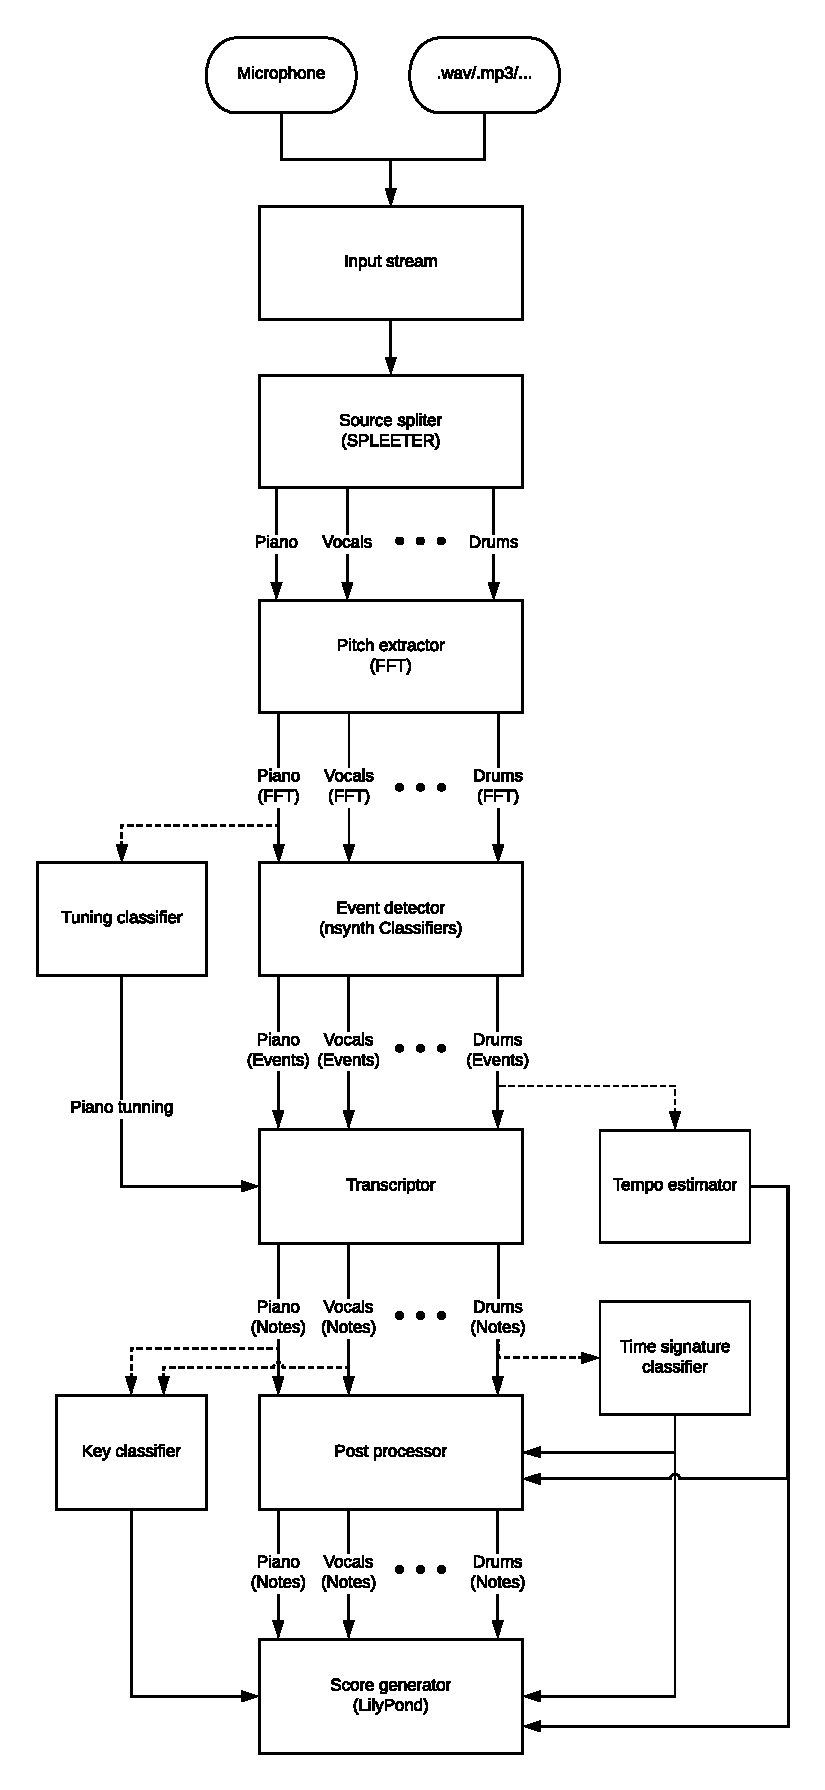
\includepdf{architecture.pdf}

\section{Audio streaming}\label{sec:audio-streaming}

This implementation directly works only with \ac{WAVE} (.wav/.wave). Any other format is converted to WAVE first,
then processed.

\subsection{WAVE format}\label{subsec:wave-format}
\textbf{WAVE} is an audio file format standard, developed by Microsoft and IBM, for storing an audio bitstream on PCs.
What's important for this thesis and implementation is that it stores data in chunks in \ac{LPCM} format. This format
allows to perform \ac{DFT} used in pitch extraction.

\subsection{Sampling rate}\label{subsec:sampling-rate}
\ac{LPCM} mentioned above stores sampled amplitude of recorded audio at specific sampling rate (frequency, measured in
Hz).

The most common sampling rate is 44.1 kHz, or 44100 samples per second. This is the standard for most consumer audio,
used for formats like CDs\cite{digital-audio-basics}.

The sampling rate determines the range of frequencies captured in digital audio. According to \textit{Nyquist Theorem},
a signal which has a Fourier transform having only frequencies upto a certain maximum $f_m$, we can obtain the analog
signal $f(t)$ from the sampled signal $f'(t)$ by passing the sampled signal $f'(t)$ through a low pass filter provided
that the sampling frequency $f_s$ is more than twice the maximum frequency $f_m$ present in the signal i.e.\ ,
$f_s > 2f_m$\cite{signals-and-systems}. Hence, having 44100 Hz sampling rate, we can reproduce and analise frequencies
up to 22050 Hz. The lowest frequency a person can hear is 20 Hz. The highest frequency humans can hear are in the range
of 20.000 Hz, but only young people can hear such high tones\cite{roots-of-modern-technology}.

The implementation is able to process input sound with any sampling rate, though lower sampling rates may cause
inaccuracies for high frequencies due to effect called \textit{aliasing}. The phenomenon of aliasing occurs if
the sampling rate is less than the Nyquist rate ($2\times$ the highest frequency). If sampling rate is less than or greater
than the Nyquist rate, it is called under sampling or over sampling. Aliasing phenomenon occurs only for under sampling.
If the sampling frequency is too low the frequency spectrum overlaps, and becomes corrupted\cite{signals-and-systems}.

\pagebreak

\section{Music source separation}\label{sec:music-source-separation}

First step of the sound processing is separation of the sound into source instruments (i.e.\ voice, guitar, piano,
etc.)

As was mentioned in previous chapter, for separation of source instruments, this implementation uses \textit{Spleeter}.
\textit{Spleeter} is a fast and state-of-the art music source separation tool with pre-trained
models\cite{spleeter2019}. Its implementation contains three pre-trained models:

\begin{itemize}
	\item vocals/accompaniment separation
	\item 4 stems separation as in \ac{SiSeC}\cite{stter20182018} (vocals, bass, drums and other)
	\item 5 stems separation with an extra piano stem (vocals, bass, drums, piano and other). It is, to the authors
	knowledge, the first released model to perform such a separation.
\end{itemize}

Estimations for all the models is performed in a frequency domain of the sound. Meaning that sound data from time domain
is converted to frequency domain using \ac{FFT}, passed to the models described in section~\ref{subsec:music-source-separation:u-net-architecture}
about U-net architecture. Output of the model is separated tracks for each instrument and voice. To get sound of each
instrument and voice in time domain (as it would be represented in \ac{WAVE}), we'd need to pass it through \ac{IDFT}.
Though it is unnecessary, as all the subsequent processing will be performed on the sound in frequency domain.

More about \ac{FFT} in the following section~\ref{sec:pitch-extraction} about pitch extraction.

\section{Pitch extraction}\label{sec:pitch-extraction}

\subsection{Multiresolution \ac{FFT}}\label{subsec:multiresolution-fft}
https://pdfs.semanticscholar.org/d55f/984d569786e1bbf945f7683361ffbbfff79a.pdf

\section{Event detection}\label{sec:event-detection}

\section{Tuning classification}\label{sec:tunning-classification}

\section{Transcription}\label{sec:transcription}

\section{Tempo estimation}\label{sec:tempo-estimation}

\section{Time signature estimation}\label{sec:time-signature-estimation}

\section{Key classification}\label{sec:key-classification}

\section{Post processing}\label{sec:post-processing}

\section{Score generation}\label{sec:score-generation}



